%----------------------------------------------------------------------------------------
%    PACKAGES AND THEMES
%----------------------------------------------------------------------------------------
\documentclass[handout, aspectratio=169,xcolor=dvipsnames]{beamer}
\makeatletter
\def\input@path{{theme/}}
\makeatother
\usetheme{CleanEasy}
\usepackage[utf8]{inputenc}
\usepackage{lmodern}
\usepackage[T1]{fontenc}
% \usepackage[brazil]{babel}
\usepackage{fix-cm}
\usepackage{amsmath}
\usepackage{mathtools}
\usepackage{listings}
\usepackage{xcolor}
\usepackage{hyperref}
\usepackage{graphicx} % Allows including images
\usepackage{booktabs} % Allows the use of \toprule, \midrule and \bottomrule in tables
\usepackage{tikz}
\usetikzlibrary{positioning, shapes, arrows, calc, decorations.pathreplacing, arrows.meta, backgrounds, patterns, overlay-beamer-styles}
\usepackage{etoolbox}
\usepackage{animate}
\usepackage{multimedia}
\usepackage{media9}

\usepackage{subfiles}
\usepackage[normalem]{ulem}
\usepackage{cancel}
\usepackage{xmpmulti}
\newcommand{\bx}{\mathbf{x}}
\newcommand{\by}{\mathbf{y}}
\newcommand{\pd}{p_\text{data}}
\newcommand{\pt}{p_\theta}
\newcommand{\nbx}{\nabla_{\bx}}

\newcommand{\btx}{\mathbf{\tilde{x}}}
\newcommand{\qs}{q_{\sigma}}
\newcommand{\nbtx}{\nabla_{\btx}}

%----------------------------------------------------------------------------------------
%    LAYOUT CONFIGURATION
%----------------------------------------------------------------------------------------
\input{configs/configs}
%----------------------------------------------------------------------------------------

% References from references.bib

\usepackage[backend=bibtex,sorting=none, style=authoryear]{biblatex}
\addbibresource{references.bib}


\begin{document}
\section{Week 8 updates}

\begin{frame}{Attempted fixes}
    \begin{itemize}
        \item Log-normal time sampling to over-emphasize intermediate times - extremely unstable sampling when trained on small number of epochs, might work with a lot more
        \item Translation of $x_1$ by $+10$ resulted in the model outputting 0
        \item Train from $x_0 \sim \mathcal{N}(0, 1)$ but clamp to $[-1, 1]$ - mostly reduces exploding outliers but results in low-diversity output
    \end{itemize}
\end{frame}


\begin{frame}{Variable-sized clouds}
    \begin{itemize}
        \item Can't find bug in zero padding
        \item Potential fix: apply curriculum learning approach. Sort training data such that average jet size per batch decreases over time
    \end{itemize}
\end{frame}

\begin{frame}{Potential fix for exploding output}
    \begin{itemize}
        \item Return $x^L - x_0$ instead of $x^L$ - when the model performs poorly and returns an identity output, we return 0 as opposed to a linearly exploding output
    \end{itemize}
\end{frame}

\begin{frame}{Rotation invariance}
    Apply approach of \cite{songEquivariantFlowMatching2023} to permute and rotate particles in $x_0 \sim \mathcal{N}$ to align with $x_1 \sim p_\text{data}$ in every $(x_0, x_1)$ training pair
    \begin{figure}
        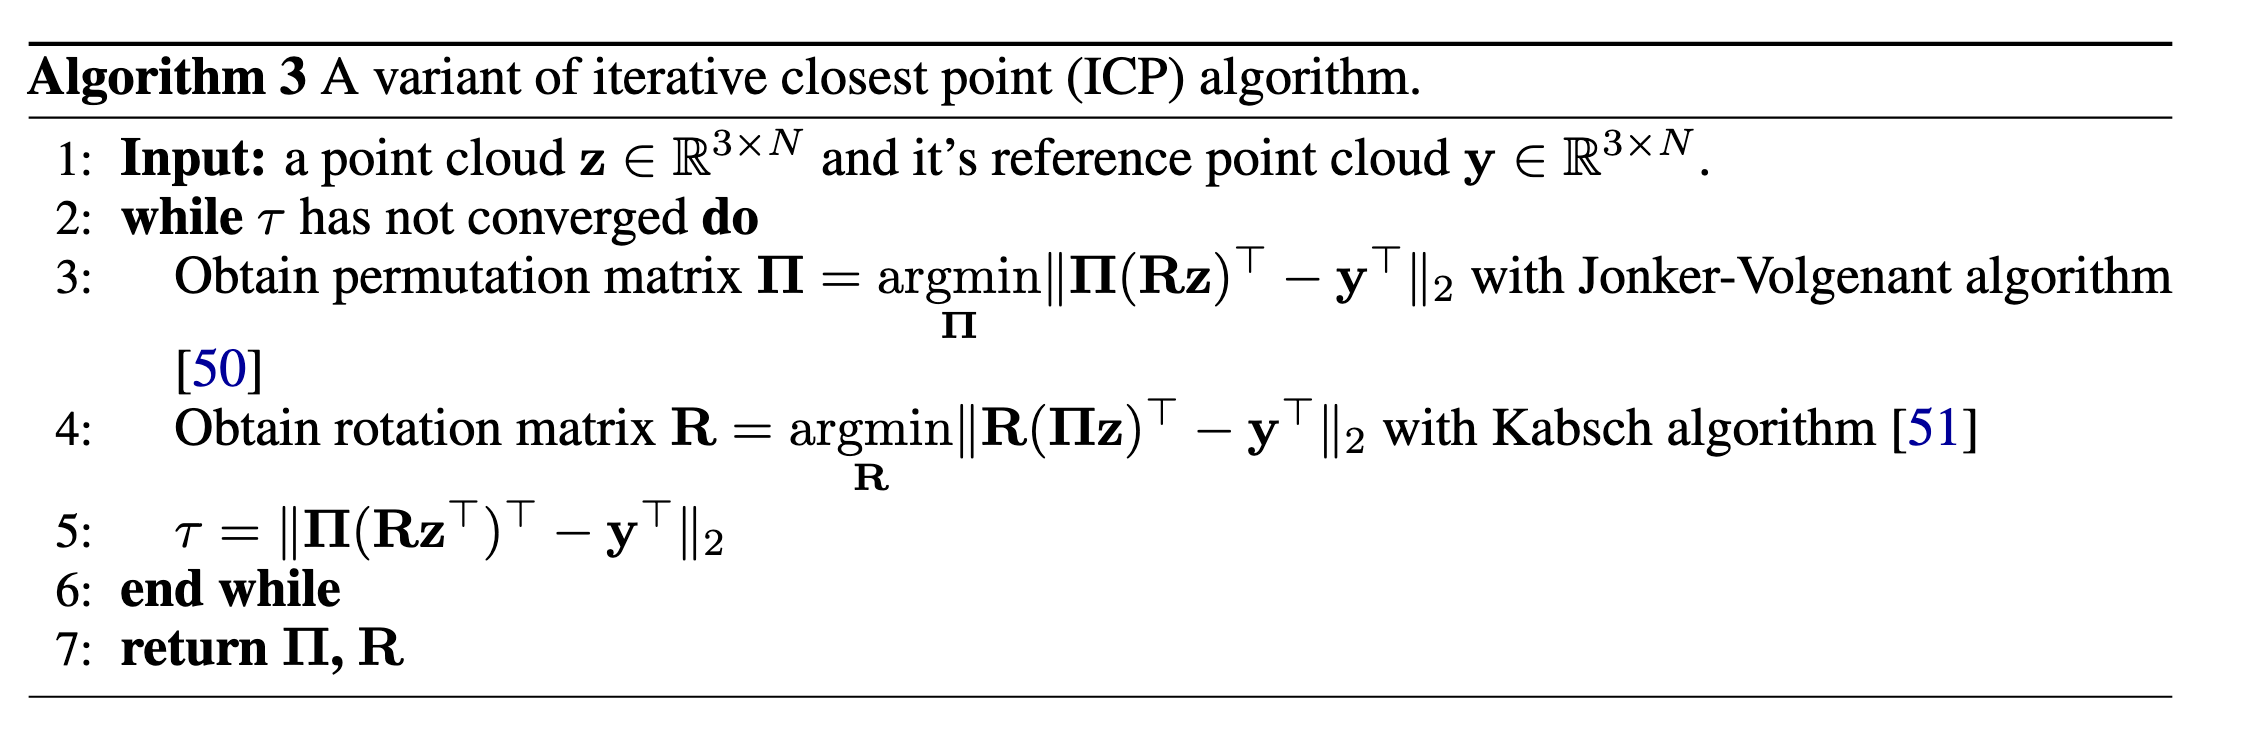
\includegraphics[height=0.5\textheight]{figs/song2023-icp.png}
    \end{figure}
    % This guarantees a rotation-invariant probability path
\end{frame}

\begin{frame}{Boost invariance}
    \begin{itemize}
        \item \cite{songEquivariantFlowMatching2023} achieve translation invariance by projecting $x_0$ to zero COM space during training, and projecting $x_t$ to zero COM at every step of the ODE solver
        \item We have the target jet's 4-momenta, so we can boost the noisy particles $x_0$ from their own reference frame to the reference frme of the jet at initialization, and similarly boost 
    \end{itemize}
\end{frame}

\begin{frame}{Cooordinate space}
    Approach of \cite{spinnerLorentzEquivariantGeometricAlgebra2024}:
    \begin{itemize}
        \item Polar coordinates are more physically meaningful than Cartesian coordinates, but working in Cartesian coordinates is better for equivariance
        \item The network works entirely in Cartesian coordinates, and its outputs are projected to polar coordinates
        \item Loss is calculated in terms of polar coordinates
        \item Should mitigate the zero-collapse issue
    \end{itemize}
\end{frame}




% \begin{frame}{Hyperparameter tuning}
%     \begin{itemize}
%         \item $\sigma_\text{min} = 10^{-4}$
%         \item Logit-normal time sampling
%         \item Smaller Xavier initialization
%         \item Bug with learning rate = 0 in late stages
%         \item Clamp $x_0 \sim \mathcal{N}(0, 1)$ to 2.5 stddevs during inferences
%     \end{itemize}
%     % Global embedding has jet $p_t$ and mass appended as scalars to deep embedding of jet type and jet # constituents
% \end{frame}

% \begin{frame}{New masking idea}
%     \begin{itemize}
%         \item Masks are a 5th feature of each particle to learn
%         \item Curriculum learning
%     \end{itemize}
% \end{frame}

% \begin{frame}[allowframebreaks]{New architecture with learnable mask flow}
%     $x$ = Cartesian particle 4-momenta, $\phi_\cdot$ = learnable functions, $\psi(\cdot) = \text{sgn}(\cdot) \log(|\cdot| + 1)$, $N = \#$ particles, $|| \cdot ||, \langle \cdot \rangle$ = Minkowski norm and inner product
%     \begin{enumerate}
%         \item Embed scalar time value to random Fourier features through two fully connected layers with 32 and 64 nodes to produce $t_\text{emb}$
%         \item Pass one-hot encoded jet type $j_t$ and number of constituents $N$ through two fully-connected layers with 32 and 64 nodes to produce global embedding $g^0$
%         \item Initialize particle cloud as 5-dimensional vectors $[x_1, \dots, x_{150}]$ where each $x_i = [E, p_x, p_y, p_z, \mu_i]$ with:
%         \begin{itemize}
%             \item 4-momentum components $(E, p_x, p_y, p_z) \sim \mathcal{N}(0,1)^4$
%             \item Initial mask $\mu_i$ from informed prior distribution based on $N$
%         \end{itemize}
%         \item Replace particles in training data with positions $> N$ in each jet with null vectors $[0, 1, 1, 1]$ (non-lightlike). Then shuffle the particles in each jet 
%         \item Stack $L$ Lorentz-group equivariant layers with mask evolution: 
%         \begin{enumerate}
%             \item Input to the $l+1$-th layer is $t_\text{emb}$, $g^0$, $g^l$, and 5D particles $x_1^l \cdots x_{150}^l$
%             \item Extract 4-momenta $\hat{x}_i^l = x_i^l[:4]$ and masks $\mu_i^l = x_i^l[4]$
%             \item Calculate messages using 4-momenta: $m_{ij}^l = \phi_e^l(\psi(||\hat{x}_i^l - \hat{x}_j^l||), \psi(\langle \hat{x}_i^l, \hat{x}_j^l \rangle), g^0, g^l, t_\text{emb})$
%             \item Cache the message aggregation $M^l = \sum\limits_{i, j = 1}^{150} (\mu_j) \phi_m^l(m_{ij}^l) m_{ij}^l$
%             \item Update the global embedding $g^{l+1} = \phi_g^l \left(g^0, g^l, t_\text{emb}, \frac{\alpha^l}{150^2} M^l \right)$ where $\phi_m^l$ outputs a scalar and $\alpha_l$ is a learnable scalar
%             \item Update 4-vectors: $$\hat{x}_i^{l+1} = \phi_w^l\left(t_\text{emb}, \frac{\beta^l}{150^2} M^l \right) \hat{x}_i^l + \gamma^l \sum\limits_{j \neq i} \mu_j \phi_x^l (g^0, g^l, t_\text{emb}, m_{ij}^l) \frac{\hat{x}_i^l - \hat{x}_j^l}{1 + ||\hat{x}_i^l - \hat{x}_j^l||} $$  where $\phi_w^l$ and $\phi_x^l$ output scalars
%             \item Update masks using Lorentz-invariant features\footnote{$\phi_\text{mask}$ uses sigmoid activations}: 
%             $$\mu_i^{l+1} =\phi_{\text{mask}}^l\left(||\hat{x}_i^l||, \mu_i^l, g^l, t_\text{emb}, \frac{1}{150}\sum_{k=1}^{150} \mu_k^l \right)$$ where the inputs are the Minkowski norm, current mask, global embedding, time embedding, and average mask value
%             \item Combine into 5D output: $x_i^{l+1} = [\hat{x}_i^{l+1}, \mu_i^{l+1}]$
%         \end{enumerate}
%         \item Apply curriculum learning by sorting training data by null particle percentage and training in stages of increasing sparsity
%         \item During inference, integrate the 5D ODE and select top-$N$ particles by mask, or select all particles with $\mu_i > 0.5$
%     \end{enumerate}
% \end{frame}

\end{document}
